\fancyfoot[R]{JL}
\section[Description]{Overall Functional Description}
The Modular Wireless Diagnostic Tool (M-WDT) is a low-cost, PC-based platform
 for performing digital and analog data acquisition and signals analysis. 
With compatible input modules, the M-WDT can serve most of a design hobbyist's 
needs in the capacity of an oscilloscope, a multichannel logic/bus analyzer, or
 other generalized sensor interface. The M-WDT runs of a lithium-ion battery, features an integrated recharger, and connects over a standard 
Bluetooth\textregistered serial link via the Serial Port Profile. The system comes with a general analog input module that consists of probes and a signal 
conditioner. 

Figure \ref{fig:overall_block} depicts a block diagram of the whole system. The input modules plug into the datapath, which routes data from them through the 
wireless link to a host PC. The power subsystem provides suitable power taps for the modules and the datapath control circuitry. 

\begin{figure}[bhp]
\caption[Block Diagram Overview]{Block Diagram of Modular Wireless Diagnostic Tool}
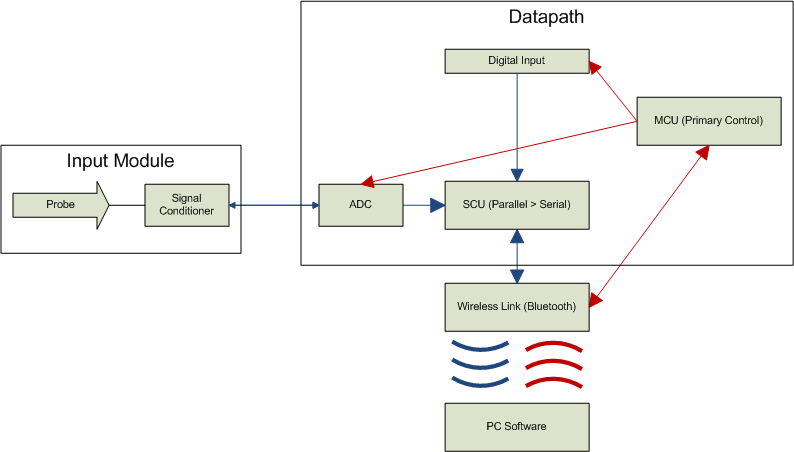
\includegraphics[width=4in]{../drawings/overview_block.png}
\label{fig:overall_block}
\end{figure}

At maximum clock speed, the M-WDT should be able to acquire data at a rate of 
250K 10-bit samples/second. This rate should be sufficient for most hobbyist needs or for field work.
